\section{Methodology}\label{sec:methods}

Tran and Yates' primary contribution lies in their approach to consider entities independently of the underlying large language model. To achieve this, they combine embeddings from an arbitrary large language model with embeddings of entities extracted from documents and queries. The embeddings of entities offer multiple views on the same information, with different sets of entities representing various perspectives on the queries and documents. Depending on the displayed view, different relevant documents or sections of documents can be identified.

Tran and Yates do not incorporate separate embeddings of queries and documents into a learned framework. Instead, they merge these embeddings into a joint vector space. This joint vector space results in a final embedding used to calculate similarities between vectors. Thus, Tran and Yates adopt the bi-encoder model (as discussed in \autoref{sec:introduction}), allowing for indexing of document embeddings and enabling fast ranking computations through ANN search. 

\subsection{General Model}\label{subsec:general_model}

Tran and Yates' proposed method involves independent embeddings of documents and entities. The process entails merging the embeddings of both documents and entities for each query and document to achieve a joint vector space, as depicted in \autoref{fig:general_model}. Following the bi-encoder approach, the embeddings for queries and documents are created independently using a pre-trained large language model.

\begin{figure}[!htb]
    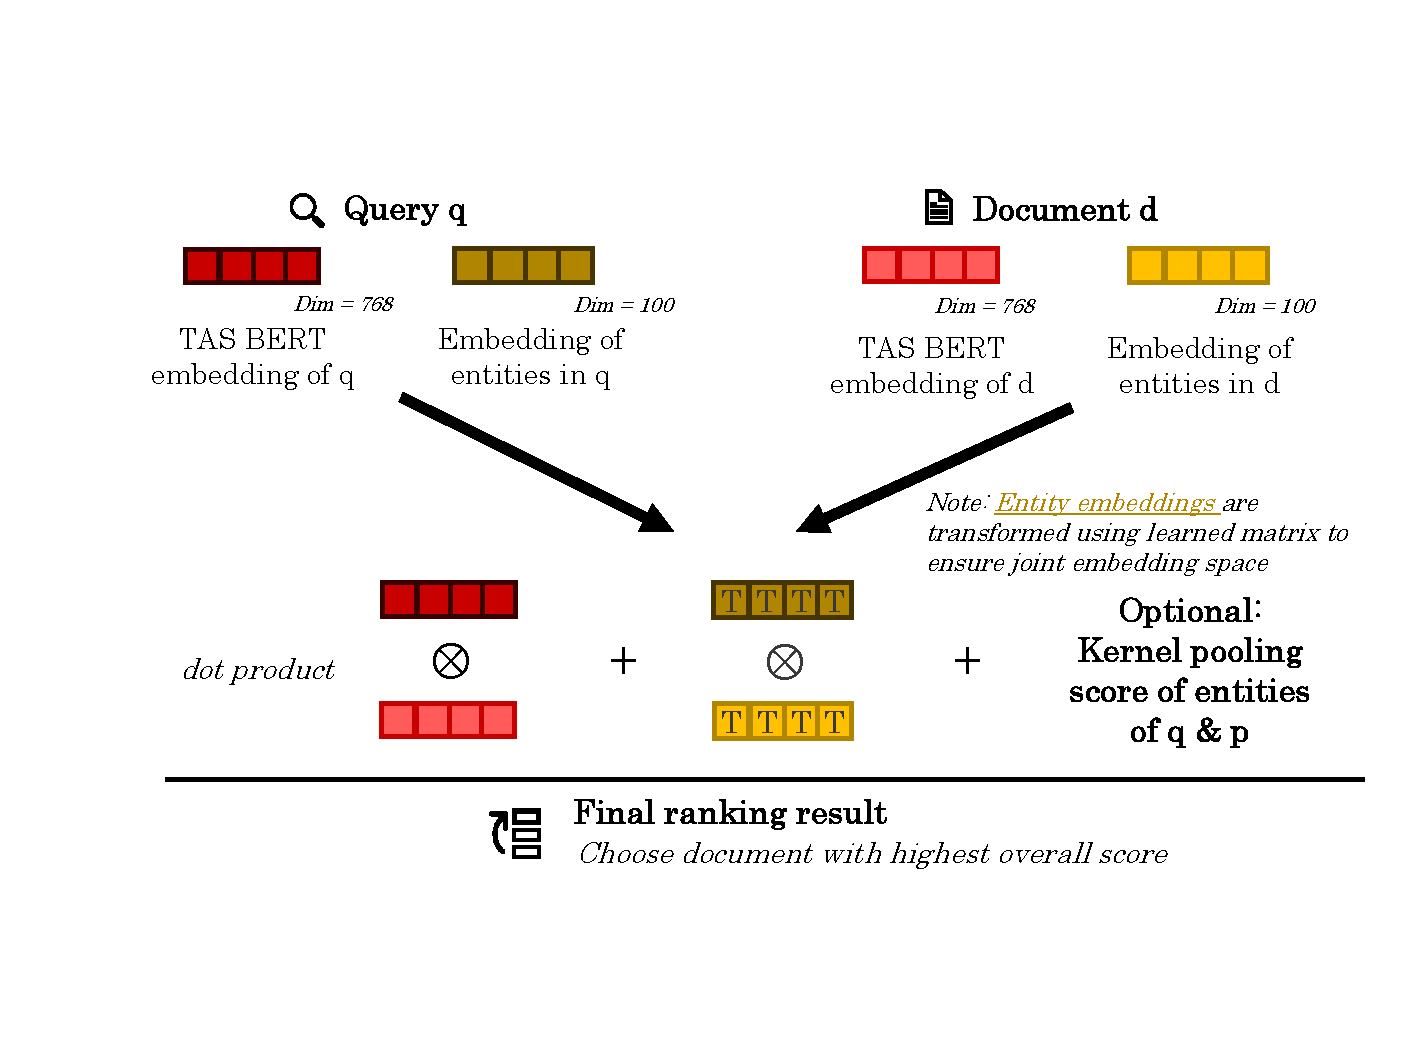
\includegraphics[trim={1.5cm 3cm 1.5cm 3cm}, clip, width=\textwidth]{resources/general_model} 
    \caption{General model}
    \label{fig:general_model}
\end{figure}

To maintain low computational costs without compromising effectiveness, Tran and Yates use a distilled version of BERT that was fine-tuned via the TAS BERT approach for information retrieval by Hofst{"a}tter et al. \cite{tasbert}.

The TAS BERT approach employs topic-aware sampling for fine-tuning on information retrieval task, thus queries in the training dataset are clustered based on different topics. During training, query samples are extracted exclusively from clusters with identical topics, aiming to enhance the sensitivity of the information retrieval model to different topics.

In the dense retrieval setting, embeddings of tokens are compared using similarity measurements to rank the best documents concerning a query. Tran and Yates follow a similar principle but enhance it by incorporating embeddings of entities. For each query and document, a single entity embedding is generated and concatenated with the textual embedding to create an embedding that captures both the semantic context and entity information.

In a usual dense retrieval setting, the generated embeddings of tokens are then compared using similarity measurements. When a query is submitted to a system, the ranking of the best documents with respect to the query is carried out, based on the calculated similarity score between the duets of the given query and all documents. 

Experimental results demonstrate that concatenation produces superior results for combining text and entity embeddings compared to other methods as max pooling and sum pooling. \autoref{tab:operator} displays the respective analysis of Tran and Yates based on their experimental setup, which is introduced in detail in \autoref{sec:results}. Apart from the analytical point of view, the approach of concatenation offers the advantage that it can be understood quite intuitively.

\begin{table}[!htb]
    \centering
    \begin{tabular}{llll}
    \hline
    \multirow{2}{*}{\textbf{Operators}} & \multicolumn{3}{c}{\textbf{MS MARCO Dev}}   \\
                                      & \textbf{nDCG} & \textbf{MRR} & \textbf{MAP} \\
    \hline
    Sum & 0.393 & 0.335 & 0.339 \\
    Max & 0.388 & 0.330 & 0.334 \\
    Concat & 0.396 & 0.341 & 0.343 \\
    \hline
    \end{tabular}
    \caption{Varying Aggregation Operators of Embedding Concatenation}
    \label{tab:operator}
\end{table}

However, concatenation introduces a challenge as the word embeddings and entity embeddings are generated in different vector spaces with varying dimensions and magnitudes. To address this issue, Tran and Yates introduce a transformation matrix $W \in \mathbb{R}^{100 \times 100}$ to transform the entity embeddings into the joint vector space.

So let $\mathbf{E}(t) \in \mathbb{R}^{100}$ be the embedding of entities of text $t$, the transformed entity embedding is given as:
\begin{align}
    \mathbf{R}_{entity}(t) = W^T \cdot \mathbf{E}(t)
\end{align}
The values of the matrix are determined during training process and thus reflect a meaningful transformation of the embeddings into a joint vector space. 

Given a text $t$ with its corresponding word embedding $\mathbf{R}_{text}(t)$ derived from the pre-trained language model, the final vector representation of $t$ is obtained by concatenating the transformed entity embedding $\mathbf{R}_{entity}(t)$ and the word embedding:
\begin{align}
\mathbf{R}_{final}(t) &= \mathbf{R}_{text}(t) \oplus \mathbf{R}_{entity}(t)
\end{align}

The ranking score value of a pair of query $q$ and document $d$ is then obtained using the dot product $\otimes$ as a similarity measure:
\begin{align}
    \mathbf{Score}(q,d) &= \left( \mathbf{R}_{final}(q) \otimes \mathbf{R}_{final}(d) \right) \\
    &= \left( \mathbf{R}_{text}(q) \otimes \mathbf{R}_{text}(d) \right) \oplus \left( \mathbf{R}_{entity}(q) \otimes \mathbf{R}_{entity}(d) \right)
\end{align}

As an optional addition to their model, Tran and Yates include an external scoring source called KNRM signal, which measures the relationship between query entities and documents. This interaction-based approach requires knowledge of the query and document at runtime. For details, consult following \autoref{subsec:knrm}.

Incorporating the KNRM signal $S_{knrm}$ into the final ranking score yields the score with KNRM signal, denoted by $\mathbf{Score}_{knrm}(q,d)$:
\begin{align}
    \mathbf{Score}_{knrm}(q,d) &= \left( \mathbf{R}_{final}(q) \otimes \mathbf{R}_{final}(d) \right) + S_{knrm}
\end{align}

\subsection{KNRM Signal}\label{subsec:knrm}

Tran and Yates introduce the KNRM signal, originally developed by Xiong et al. \cite{xiong2017end}, as an additional scoring mechanism to extend their basic approach by a separate framework. Unlike its original use, Tran and Yates adapt the KNRM model to specifically capture the interaction between entities in queries and documents. The calculation of the KNRM signal follows these steps:

\begin{enumerate}
    \item Let $X(q)$ be the set of all entity embeddings within query $q$, $X(d)$ any set of entity embeddings which occur in document $d$. For EVA Single and EVA Single-QA models (see \autoref{subsec:models}) $X(d)$ contains all entities with the given document, for EVA Multi (see \autoref{subsec:models}) $X(d)$ contains only entities of specific subsets of entities of $d$. The entity interaction matrix is defined as: 
    \[T_{i,j} := sim(X_i(q), X_j(d)) \text{~,}\]
    where $X_i(q)$ and $X_j(d)$ are the $i$-th and $j$-th embedding of $q$ and $d$. The similarity function is given as cosine similarity. Embeddings are generated via Wikipedia2Vec (Yamada et. al \cite{yamada2018wikipedia2vec}), as described in \autoref{subsubsec:extracting_entities}.
    \item Build k kernels using radial basis function, which creates differentiable histograms around given $\mu$ and $\sigma^2$.
    \[ K_l(X_i(q)) = \sum_{j=1}^{|X(p)|}\exp\left(-\frac{(T_{i,j}-\mu_i)^2}{2\sigma_i^2}\right)\]
    \item Pool / Summarize the k results into a k-dimensional feature vector: \[\overrightarrow{K(X_i(q))} = [K_1(X_i(q)), \ldots, K_k(X_i(q))]\]
    \item Build kernel-pooled representation $\phi(T)$ by calculating log-sum for each query entity: \[\phi(T) = \sum_{i=1}^{|X(q)|} \log \overrightarrow{K(X_i(q))}\]
    \item Get final kernel pooling score by applying a learned ranking layer. Note that $\tanh(\cdot) \in (-1, 1)$ and therefore $\sup S_{knrm} = 1$: \[ S_{\text{knrm}} = \tanh(w^T\phi(T) + b) \]
  \end{enumerate}

Despite being an interaction-based model that requires scoring during runtime for all query-document pairs, the computational complexity of the KNRM approach remains limited. The computations involved are relatively straightforward, and the additional learned layer does not significantly increase the computational overhead. Furthermore, these computations can be performed in parallel with the other components of Tran and Yates' approach. Empirical results concerning the latency of the models, with and without the KNRM signal, validate this assertion (see \autoref{sec:results}).

\subsection{Generating Entity Embeddings\label{subsec:entity_embeddings}}

As described in \autoref{subsec:general_model}, Tran and Yates create embeddings for both word tokens and entities in queries and documents. While the word token embeddings are generated using pre-trained TAS BERT, the primary focus of the contribution of Tran and Yates lies in the creation of entity embeddings. In particular, as queries and documents often contain multiple entities, these entities need to be aggregated into a single embedding.

To illustrate this process, consider the example depicted in \autoref{fig:example}. In this example, the query 'Favourite book bert sesame street' corresponds to a document that mentions three entities: Bert, Sesame Street and Boring Stories.

\begin{figure}[!htb]
    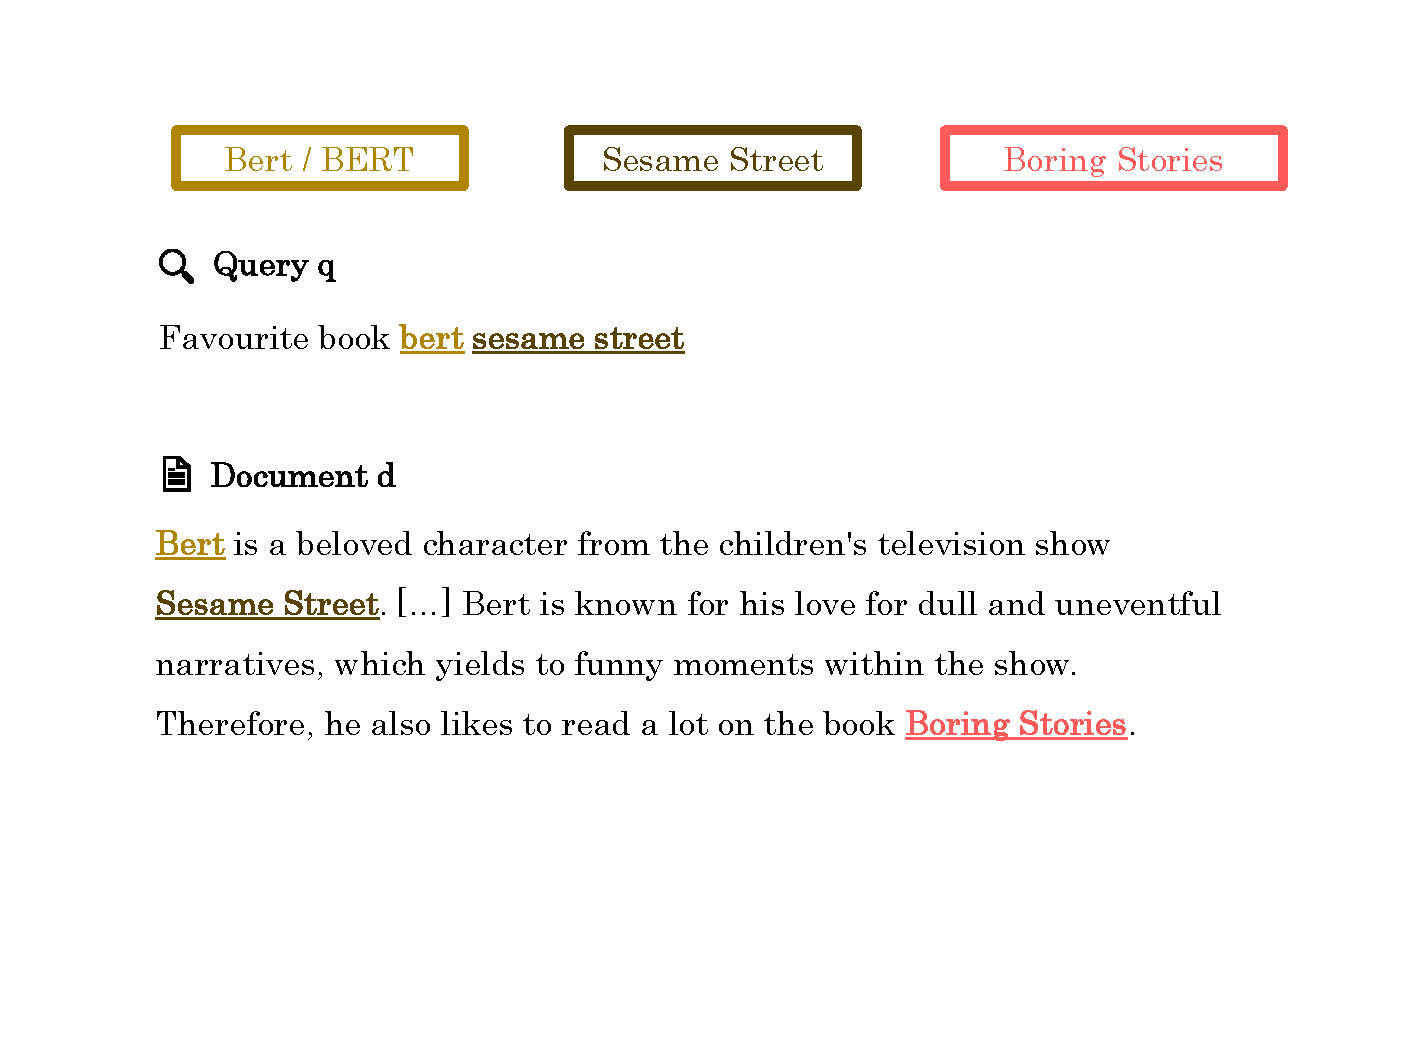
\includegraphics[trim={1.5cm 5.5cm 1.5cm 2cm}, clip, width=\textwidth]{resources/example} 
    \caption{Example query and example document}
    \label{fig:example}
\end{figure}

\subsubsection{Extracting Entities}\label{subsubsec:extracting_entities}

To aggregate multiple entities in a document or query, Tran and Yates first extract these entities from the text using external frameworks Dexter (Ceccarelli et al. \cite{ceccarelli2013dexter}) and Wikipedia2Vec (Yamada et. al \cite{yamada2018wikipedia2vec}).
\begin{itemize}
    \item The Dexter framework is an entity linkage system that resolves entity mentions in text to corresponding entities in a knowledge base. In particular, Dexter employs a combination of methods, including named entity recognition and pattern matching, to perform this task. 
    \item Wikipedia2Vec leverages the structure of Wikipedia to generate dense vector representations (embeddings) for words, articles, and entities. It utilizes the Word2Vec algorithm (Mikolov et al. \cite{mikolov2013distributed}) to capture semantic relationships from Wikipedia, producing high-dimensional embeddings.
\end{itemize}

The extraction procedure involves submitting a document or query to Dexter, which extracts entity mentions from the given text. These entity names are then passed on to the knowledge base, which transforms them into embeddings. Wikipedia2Vec provides vectors in dimension 100 as default, Tran and Yates keep this value in their model. \autoref{fig:entity_extraction} visualizes this process.

\begin{figure}[!htb]
    \centering
    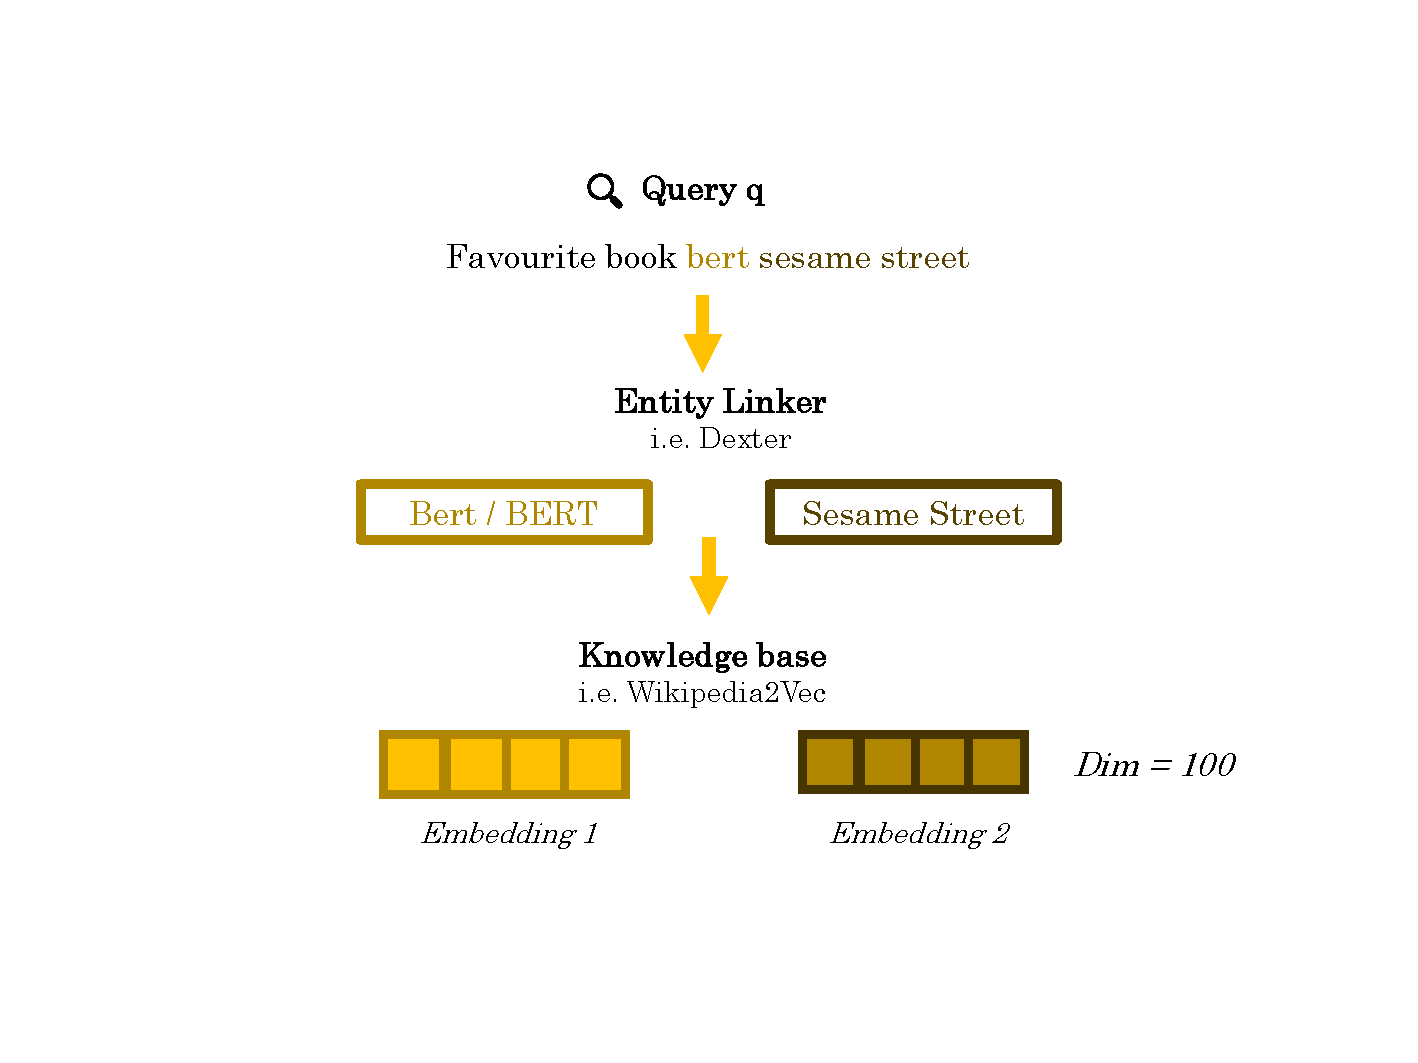
\includegraphics[trim={2cm 3cm 2cm 2cm}, clip, width=0.8\textwidth]{resources/entity_extraction} 
    \caption{Process of entity extraction}
    \label{fig:entity_extraction}
\end{figure}

\subsubsection{Combining Entities for Queries}\label{subsub:generating_queries}

For now, multiple embeddings for each entity within a query or a document are generated by applying the procedure outlined in \autoref{subsubsec:extracting_entities}. The aggregation of these generated embeddings differs based on whether a query or a document is considered, given the usual brevity of queries compared to documents.

For queries, Tran and Yates adopt a straightforward approach. They aggregate the embeddings of entities by averaging all entity embeddings across all dimensions. \autoref{fig:queries} visualizes this procedure.

\begin{figure}[!htb]
    \centering
    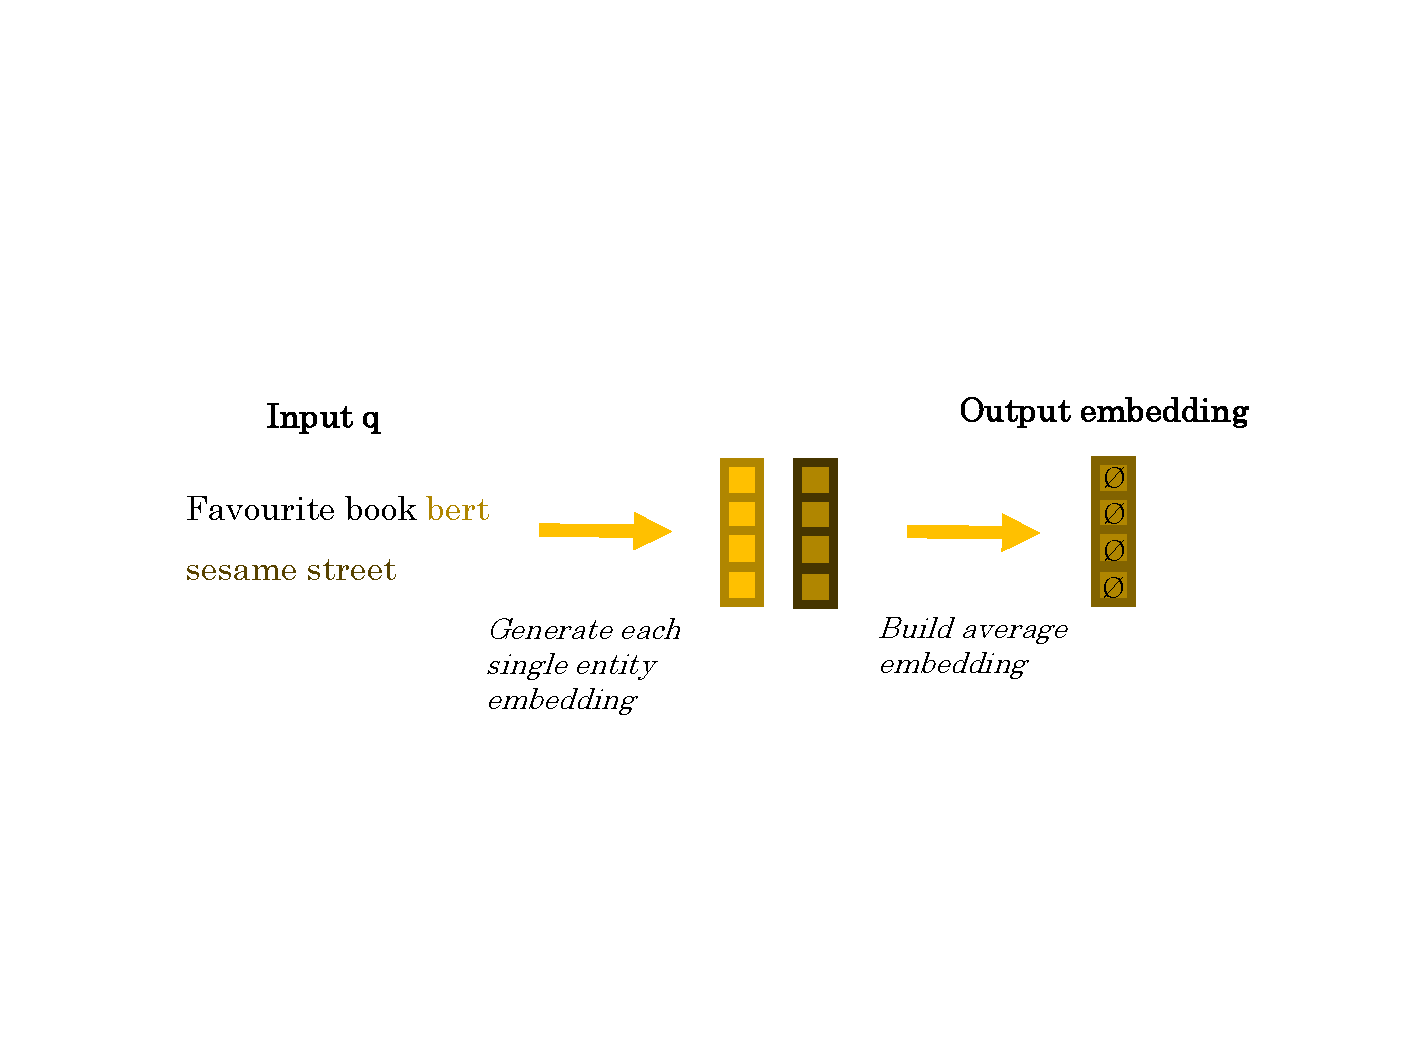
\includegraphics[trim={2cm 6cm 2cm 6cm}, clip, width=0.8\textwidth]{resources/queries} 
    \caption{Process of generating a single entity embedding for a query}
    \label{fig:queries}
\end{figure}

\subsubsection{Combining Entities for Documents}\label{subsec:models}

Documents usually contain many different entities, as the example in \autoref{fig:example} indicates. Additionally, documents might also cover different aspects of a topic, so entities from very different areas might appear within them. To handle this additional complexity, the authors proposed three successive methods for entity aggregation in documents, namely:

\begin{itemize}
    \item Single Entity Representation (EVA Single)
    \item Query-Aware Single Entity Representation (EVA Single-QA)
    \item Multiple Entity View Representation (EVA Multi)
\end{itemize}

The term 'EVA' stands for \underline{E}ntity \underline{V}iews in Dense Retriev\underline{a}l. The concept of 'Entity Views' which gives the paper its name, is particularly relevant in the third method, EVA Multi, and will be elaborated in the following sections.

\paragraph*{EVA Single}

 The key idea behind the Single Entity Representation is to extract all entities present in the document and subsequently generate a single output embedding by computing the average of these entity embeddings. This process is analogous to the one depicted in \autoref{fig:queries} for queries, and a visual representation for documents is illustrated in \autoref{fig:eva_single}.

The initial approach for aggregating entities in a document, called EVA Single, is similar to the one used for queries. The key idea behind the Single Entity Representation is to extract all entities present in the document and subsequently generate a single output embedding by computing the average of these entity embeddings. This process is analogous to the one depicted in \autoref{fig:queries} for queries, and a visual representation for documents is illustrated in \autoref{fig:eva_single}.

\begin{figure}[!htb]
    \centering
    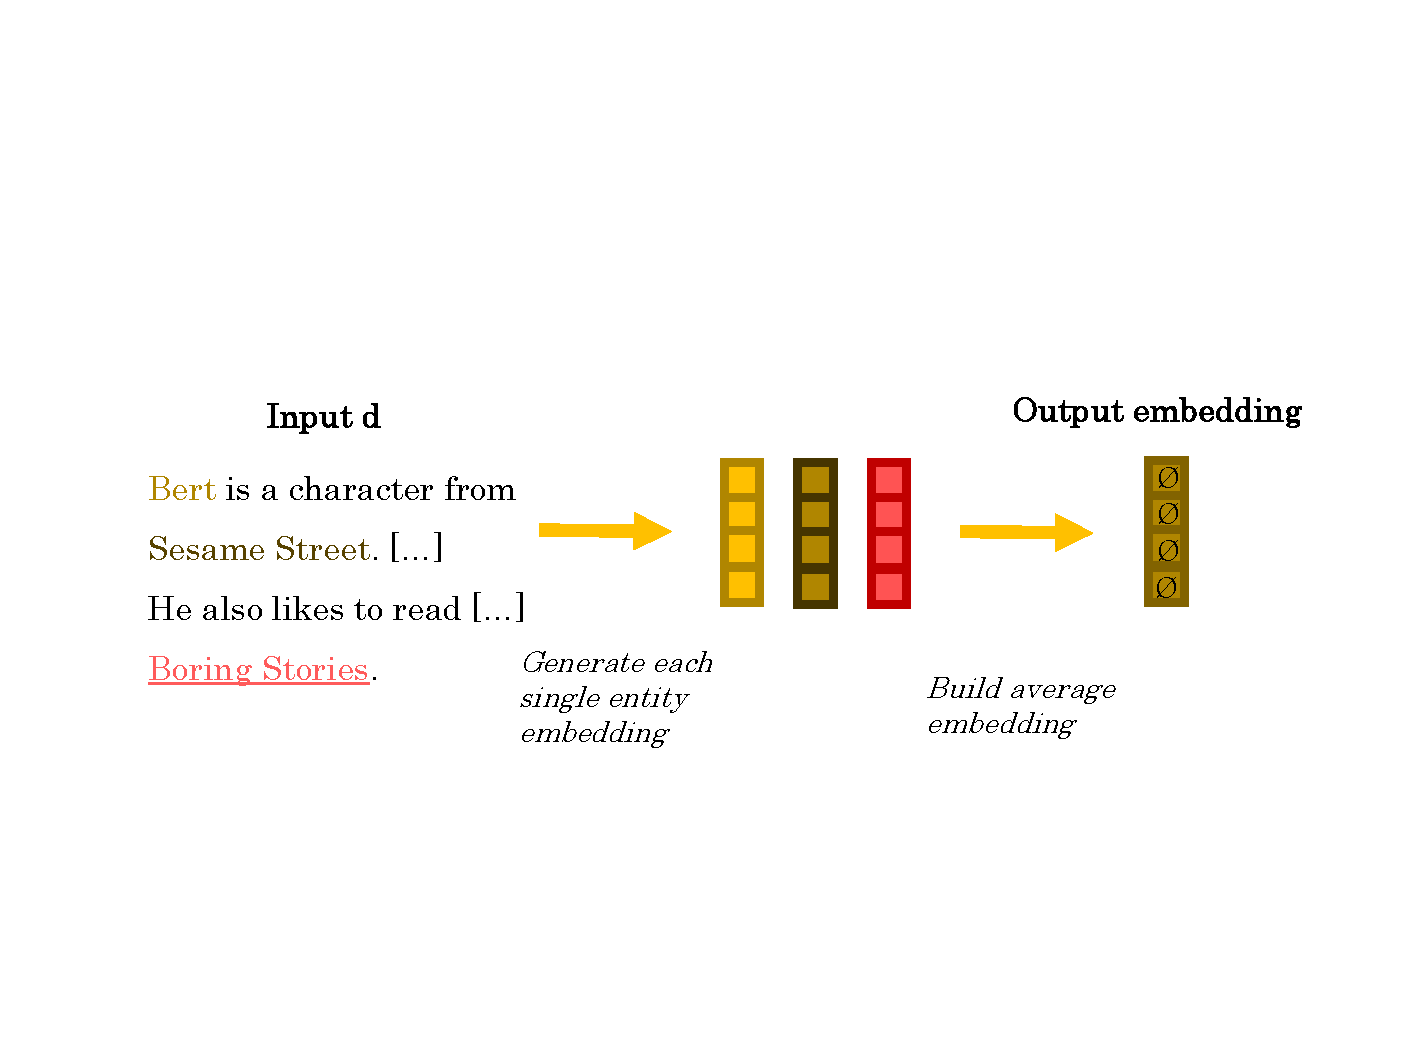
\includegraphics[trim={2cm 5cm 1.5cm 6cm}, clip, width=0.8\textwidth]{resources/eva_single} 
    \caption{Process of generating an entity embedding for a document following the EVA Single approach}
    \label{fig:eva_single}
\end{figure}

Despite its simplicity, this approach overlooks the fact that documents may cover diverse topics. By discarding query information, the EVA Single approach considers all entities, including those that may be only partially relevant to the document's main topic. Consequently, this disregards the relevance of entities within the ranking process, leading to biased results, as observed in \autoref{sec:results}.

\paragraph*{EVA Single-QA}

To address this problem, Tran and Yates introduce the Query-Aware Single Entity Representation, which creates embeddings that are tailored to the specific needs of a given query.  However, this improvement comes with increased computational complexity since it assumes knowledge of the query beforehand. As a result, calculations for all query-document pairs must be performed during runtime, eliminating the possibility of precomputing document embeddings and indexing, leading to higher latency, as observed in \autoref{sec:results}.

The underlying idea of the EVA single QA model is to filter the entities of a document based on the information of a given query and select only entities with high similarity to a query entity. \autoref{fig:eva_single_qa} visualizes this process.

\begin{figure}[!htb]
    \centering
    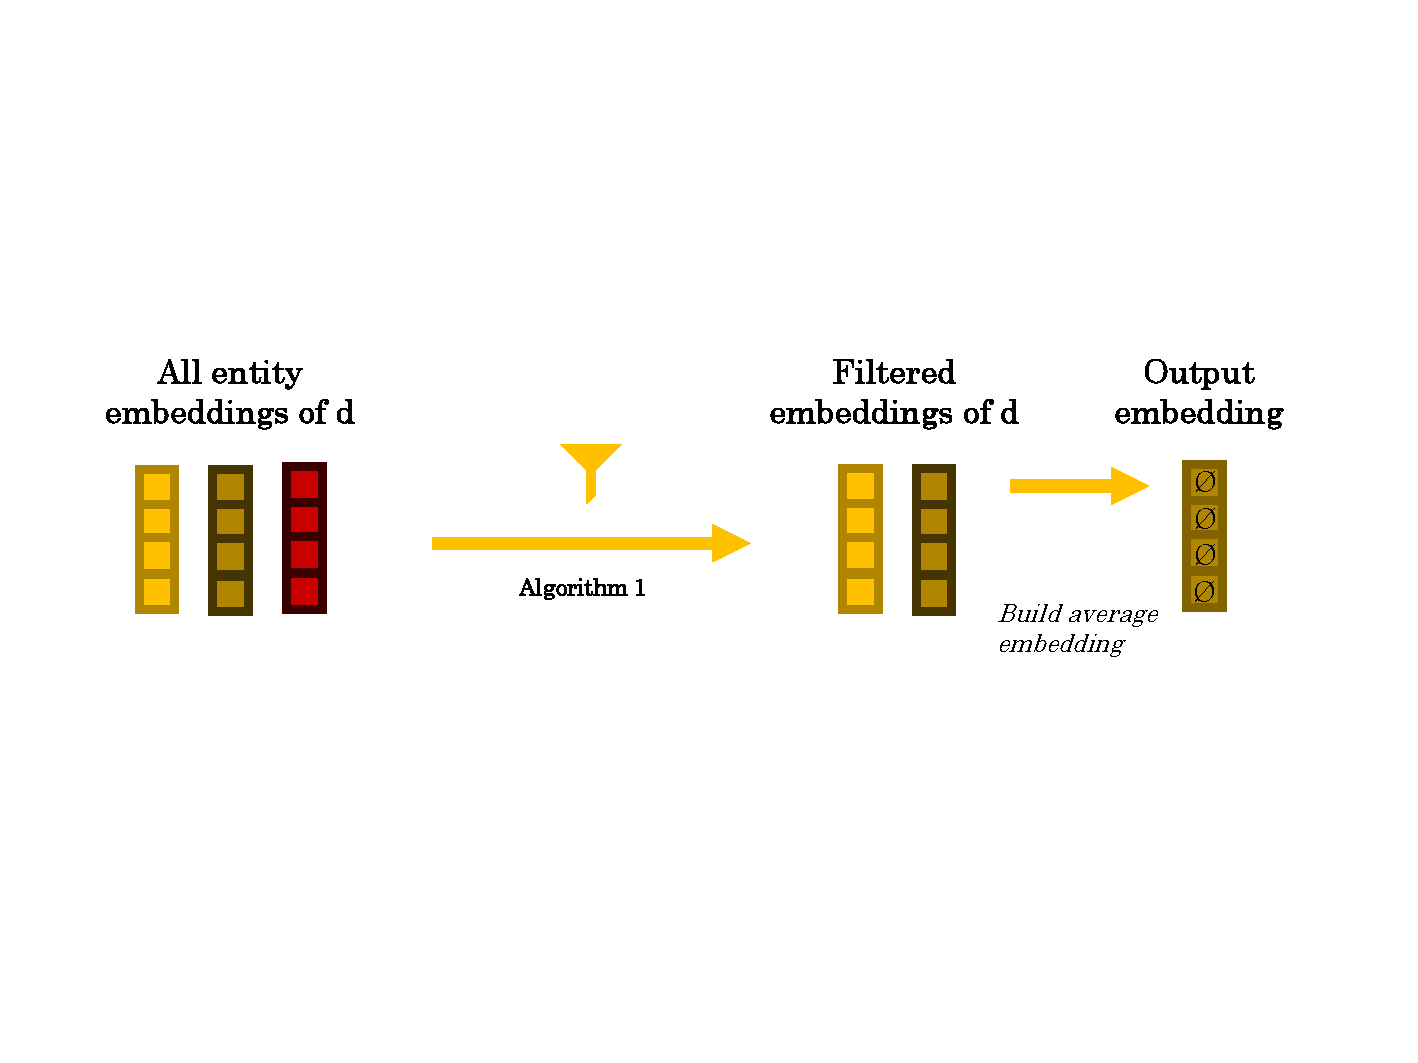
\includegraphics[trim={1cm 6.5cm 2cm 6cm}, clip, width=0.8\textwidth]{resources/eva_single_qa} 
    \caption{Process of generating an entity embedding for a document following the EVA Single-QA approach}
    \label{fig:eva_single_qa}
\end{figure}

The filtering is conducted using Algorithm \ref{alg:query-aware-entity-representation}, which is applied to each query-document pair ($q$, $d$). For every entity within $q$, the algorithm searches for the corresponding entity in $d$ that possesses the maximum cosine similarity. If the similarity exceeds a specified threshold $\alpha$, the respective entity in $d$ is added to the filtered list $X_{focus}(d)$. Subsequently, the single output embedding for document $d$ is computed as the average of all entity embeddings within $X_{focus}(d)$.

\begin{algorithm}[!htb]
    \caption{Query-aware document entity representation}
    \label{alg:query-aware-entity-representation}
    \begin{algorithmic}[1]
    \REQUIRE Query $q$ and document $d$, threshold $\alpha$
    \ENSURE Filtered entity embedding list $X_{focus}(d)$ of $d$
    
    \STATE $X(q) \leftarrow$ set of embeddings of entities in $q$
    \STATE $X_{focus}(d) \leftarrow \{\}$
    \FOR{$e$ in $X(q)$}
        \STATE $e^* \leftarrow$ entity embedding in $d$ having the maximum cosine similarity with $e$
        \IF{cosine similarity$(e^*, e) > \alpha$}
            \STATE $X_{focus}(d) \leftarrow X_{focus}(d) \cup \{e^*\}$
        \ENDIF
    \ENDFOR
    \RETURN $X_{focus}(d)$
    \end{algorithmic}
\end{algorithm}

\paragraph*{EVA Multi}

To address the issue of known queries required by the EVA Single-QA approach, Tran and Yates propose the EVA Multi method, which introduces multiple entity views as a solution with minimal negative consequences.

Analysis training data revealed that in the vast majority of instances, the number of entities in queries does not exceed two. For instance, in the MS Marco Dev dataset, 99.6 \% of the 300,000 training instances and 99.5 \% of the test instances contain two or fewer entities. Based on this observation, Tran and Yates focused their research on the assumption that it is sufficient to consider a maximum of two entities in queries.

\begin{table}[!htb]
    \centering
    \small
    \begin{tabular}{lp{2cm}cp{2cm}c}
    \hline
    \multirow{2}{*}{\textbf{Entities}} & \multicolumn{2}{c}{\textbf{Training Queries}} & \multicolumn{2}{c}{\textbf{Testing Queries}} \\
                                 & \textbf{Count}           & \textbf{Fraction}          & \textbf{Count}           & \textbf{Fraction}          \\
    \hline
    0 & 130,353 & 0.435 & 3,442 & 0.483 \\
    1 & 149,073 & 0.497 & 3,232 & 0.454 \\
    2 & 19,207 & 0.064 & 416 & 0.058 \\
    3+ & 1,367 & 0.004 & 37 & 0.005 \\
    \hline
    \textbf{Total} & 300,000 &  & 7,127 &  \\
    \textbf{Average} & 0.640 &  & 0.587 &  \\
    \hline
    \end{tabular}
    \caption{Summary statistics of the queries.}
    \label{tab:query_statistics}
\end{table}

Under this assumption, when applying Algorithm \ref{alg:query-aware-entity-representation}, at most two entities remain in the filtered embedding list $X_{focus}$. This limitation stems from the algorithm iterating over the set of all entities in the given query once, resulting in $X_{focus}$ containing either zero, one, or at most two items. The number of all possible sets eligible for $X_{focus}$ is restricted to $|\{\}| + |X(d)| + \binom{|X(d)|}{2}$, where $|X(d)|$ corresponds to the number of entities in document $d$.

Leveraging this observation, Tran and Yates introduce clusters of entities, which represent different views of a document. In the EVA Multi approach, all possible single itemsets and sets of pairs of the entities are generated. However, sets of pairs are considered only if the cosine similarity between the two entities within a pair exceeds a predefined threshold $\beta$, ensuring only relevant entity views are generated. The final output embeddings are then calculated by averaging the embeddings of all items within each set. When applying the optional KNRM signal (see \autoref{subsec:knrm}) to this approach, the entity interaction matrix $T$ is built only upon the set of entity embeddings within a single cluster, rather than considering all entities within the document.

\begin{figure}[!htb]
    \centering
    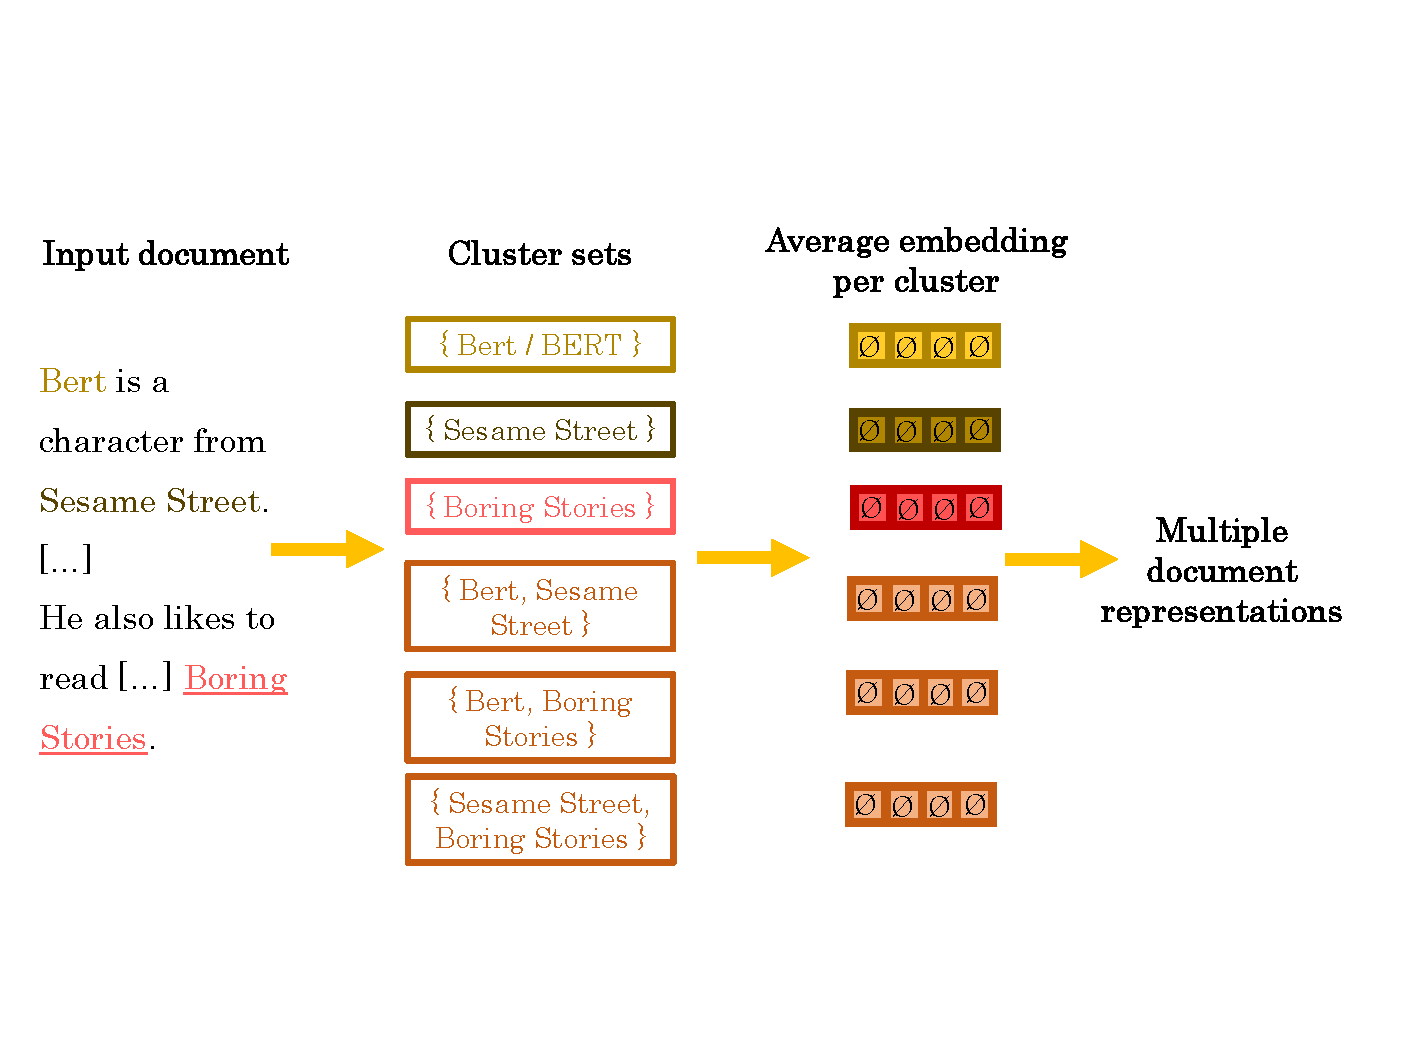
\includegraphics[trim={0cm 3cm 0cm 3.5cm}, clip, width=\textwidth]{resources/eva_multi} 
    \caption{Process of generating entity embeddings for a document following the EVA Multi approach}
    \label{fig:eva_multi}
\end{figure}

This allows all calculations to be performed independently of query information, enabling indexing. Unlike the previous methods, EVA Single and EVA Single-QA, the EVA Multi approach generates several entity output embeddings per document.

\autoref{fig:eva_multi} visualizes the process of generating the embeddings of multiple entity views or clusters. For the given example of three entities within an input document, six different views on entities and document entity representations are generated.


